\pagebreak
\section{Inertia Test}
\nopagebreak
%\subsection{} %\label{put a label here and uncomment}
\textbf{Name: Group 510}\\
\textbf{Date: 02/11 - 2015}

\subsubsection{Purpose}
The purpose of the test is to measure the inertia of the vehicle, $J_{tot}$, and the vehicle's step-response.

\subsubsection{Theory}
The \figref{inertiaTestPowerCutOrDisable} shows the vehicle's velocity variations throughout time, both when the motor is unplugged manually or when its power is cut via software :

\begin{figure}[H]
  \centering
  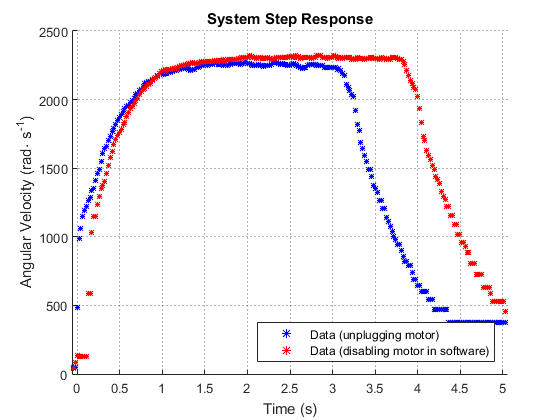
\includegraphics[scale=0.8]{figures/inertiaTestPowerCutOrDisable.png}
  \caption{Plot of the systems step-response, which is angular velocity over time. The blue dots represents the measured data when the plus-pole of the motor is unplugged manually to stop the vehicle. The red dots represents the measured data when the software is used to stop the vehicle.}
  \label{inertiaTestPowerCutOrDisable}
\end{figure}

By comparing both methods to cut off the motor's power, the back electromotive force generated by the motor when using the software method seems negligible since both curves have very similar decreasing shapes. Moreover, the manual unplugging of the powering wires brings some uncertainty due to a potential disturbance of the force applied to the vehicle.
Therefore, the software method is used to extract the inertia.
red sharper than blue

\subsubsection{Setup}
\begin{figure}[H]
	\centering
	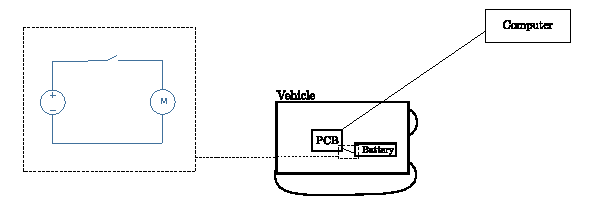
\includegraphics[scale=1.6]{figures/inertiaTestSetupDiagram.pdf}
	\caption{Setup diagram}
	\label{inertiaTestSetupDiagram}
\end{figure}

\subsubsection{List of Equipment}

\begin{table}[H]
\begin{tabular}{|p{10cm}|p{4cm}|}
\hline%------------------------------------------------------------------------------------
  \textbf{Instrument}                     &  \textbf{Type}       \\
\hline%------------------------------------------------------------------------------------
  Computer                                &  Asus N73JN    \\
\hline %-----------------------------------------------------------------------------------
\end{tabular}
\end{table}

\subsubsection{Procedure}

\begin{enumerate}
  \item Disconnect the battery.
  \item Connect the Arduino to the computer.
  \item Upload the test code to the Arduino board using the Arduino IDE  \cite{ArduinoIDE}.
  \item Open a serial terminal via PuTTY \cite{PuTTY}.
  \item Plug in the battery immediately after opening the terminal.
  \item Wait two seconds then follow the vehicle with the connected computer.
  \item Wait until the vehicle stops before ending the measurements by unplugging the connected computer from the Arduino.
  \item Plot the speed of the vehicle using Matlab.
\end{enumerate}

\subsubsection{Results} \label{inertiaTestResults}

\begin{figure}[H]
  \centering
  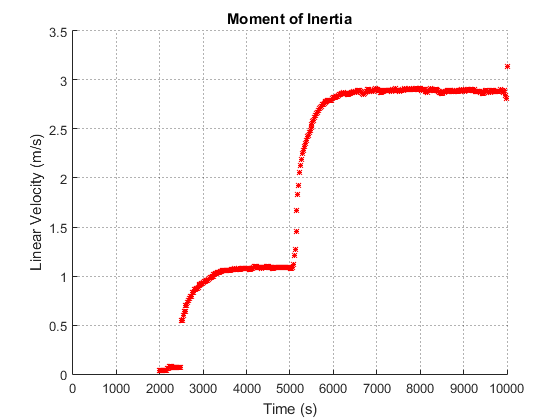
\includegraphics[scale=0.8]{figures/VehicleMomentOfInertiaTest.png}
  \caption{g}
  \label{inertiaTestPowerCutOrDisable}
\end{figure}

